Nous avons choisi le thème \textit{Rendu temps réel de scènes complexes et interaction dans un navigateur}, où il est question de générer aléatoirement un monde "Lego" virtuel et de pouvoir intéragir avec. 

Ce type de rendu est largement utilisé dans bon nombres de domaines, surtout dans le jeu vidéo où il s'impose comme une norme. Le côté aléatoire apporté par le bruit de Perlin tend à favoriser le renouvellement des environnements de jeu, et à donner un côté unique à chaque génération de la carte. L'intérêt pour nous est de nous pencher sur la façon dont ces univers sont construits, et de nous approprier les technologies les plus en vogue dans ce type de projet.

Nous avons déjà une vision précise du résultat final de ce projet. Nous souhaiterions recréer un programme capable de génrer un univers tout en 3D, généré avec le bruit de Perlin (voire avec son successeur, amélioré et plus moderne, le bruit de Simplex), dans lequel l'utilisateur peut déplacer un personnage. D'autres fonctinnalités supplémentaires pourraient également s'ajouter au projet dans le cas où nous parviendrions à remplir nos objectifs avant la date buttoir, comme par exemple l'adaptation des textures en fonction de l'altitude, l'ajout de l'eau, de différents types de reliefs, etc. 

Pour mener à bien ce projet, nous nous appuyons notamment sur l'API three.JS, écrite en JavaScript et particulièrement documentée car populaire dans le milieu de la génération des rendus en 3D.

\begin{center}
	\null\vspace{0.25cm}
	
\includegraphics[height=3cm]{images/logo-threeJS.eps}\\
	\textit{Image 1. Logo de l'API three.JS}\\
\end{center}

\newpage
Le tout sera couplé avec une page HTML, et une feuille de style. L'HTML lie la feuille de style CSS et le script en JavaScript, éxécuté par le client web pour afficher notre monde virtuel.


\begin{center}
	\null\vspace{0.25cm}
	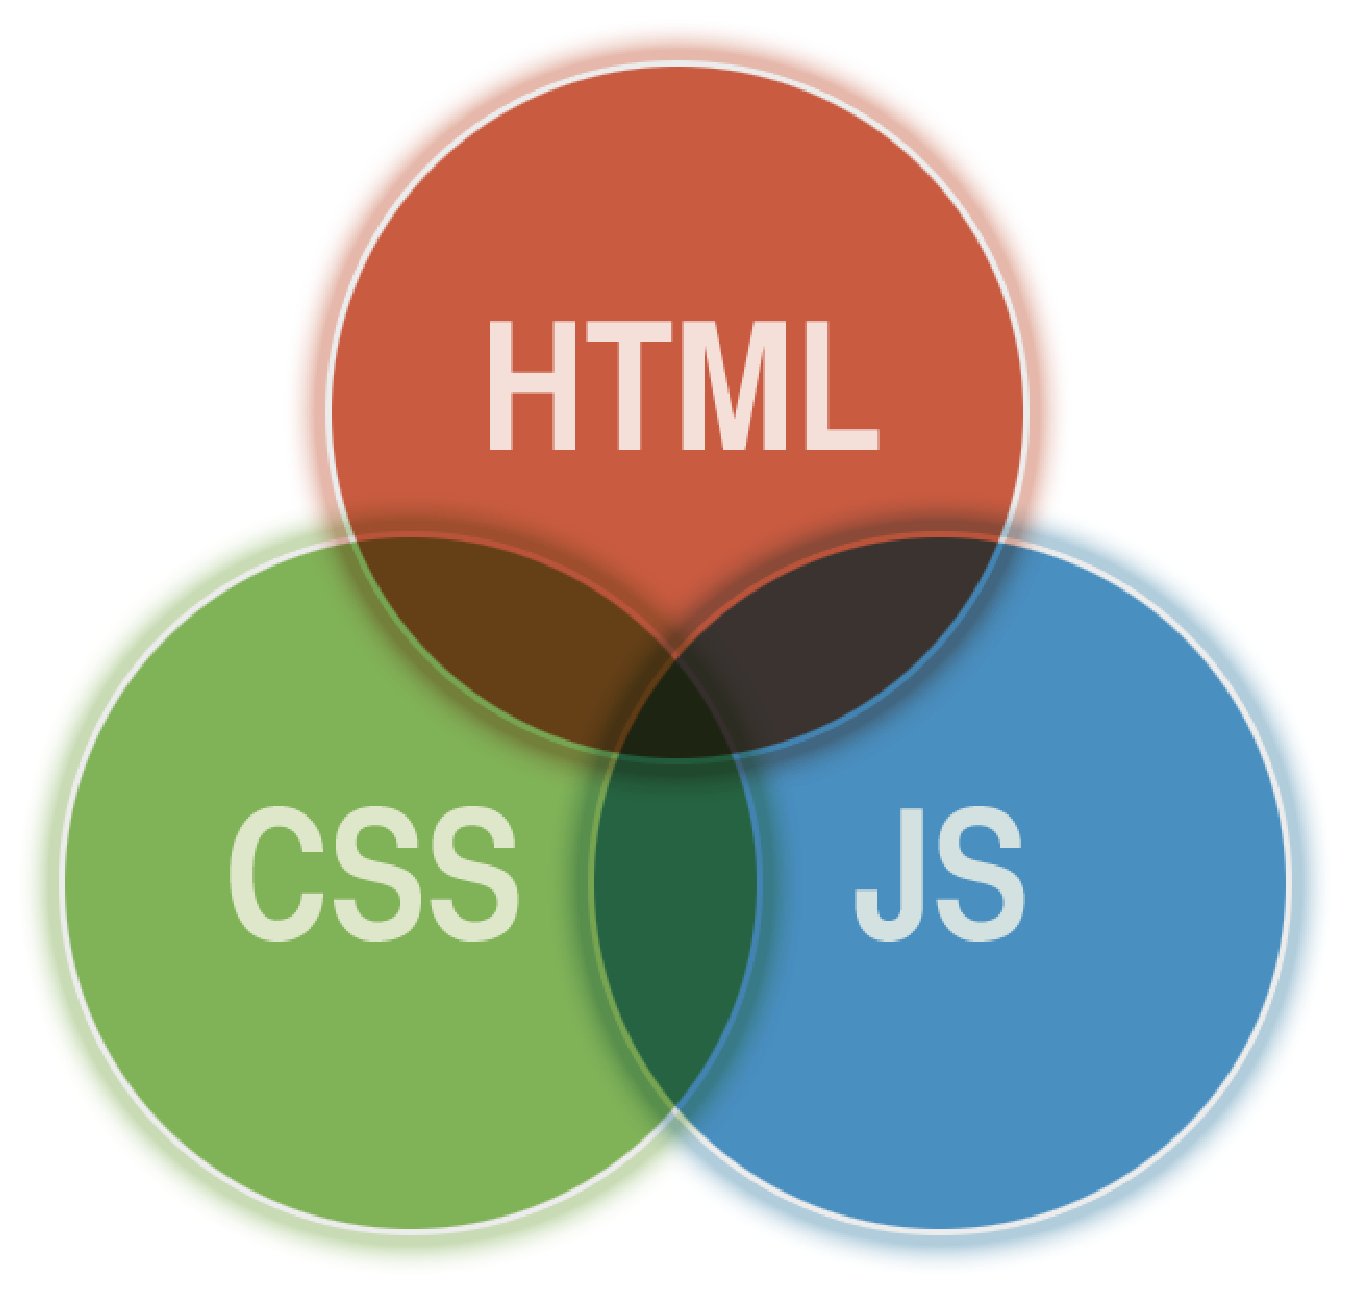
\includegraphics[height=3cm]{images/HTML-CSS-JS.eps}\\
	\textit{Image 2. Schéma des technologies utilisées}\\
\end{center}

